\chapter{研究方法}
\section{研究設計與流程}
測試文字我想畢業測試文字我想畢業測試文字我想畢業測試文字我想畢業測試文字我想畢業測試文字我想畢業測試文字我想畢業測試文字我想畢業測試文字我想畢業測試文字我想畢業測試文字我想畢業測試文字我想畢業測試文字我想畢業測試文字我想畢業測試文字我想畢業測試文字我想畢業測試文字我想畢業測試文字我想畢業測試文字我想畢業測試文字我想畢業測試文字我想畢業測試文字我想畢業測試文字我想畢業測試文字我想畢業測試文字我想畢業測試文字我想畢業測試文字我想畢業測試文字我想畢業測試文字我想畢業測試文字我想畢業測試文字我想畢業測試文字我想畢業測試文字我想畢業測試文字我想畢業測試文字我想畢業測試文字我想畢業測試文字我想畢業測試文字我想畢業測試文字我想畢業測試文字我想畢業測試文字我想畢業測試文字我想畢業測試文字我想畢業測試文字我想畢業測試文字我想畢業測試文字我想畢業測試文字我想畢業測試文字我想畢業測試文字我想畢業測試文字我想畢業測試文字我想畢業測試文字我想畢業測試文字我想畢業測試文字我想畢業測試文字我想畢業測試文字我想畢業測試文字我想畢業測試文字我想畢業測試文字我想畢業測試文字我想畢業

本研究吉祥物如圖~\ref{i:cat}。
\begin{figure}[!htbp]
\centering
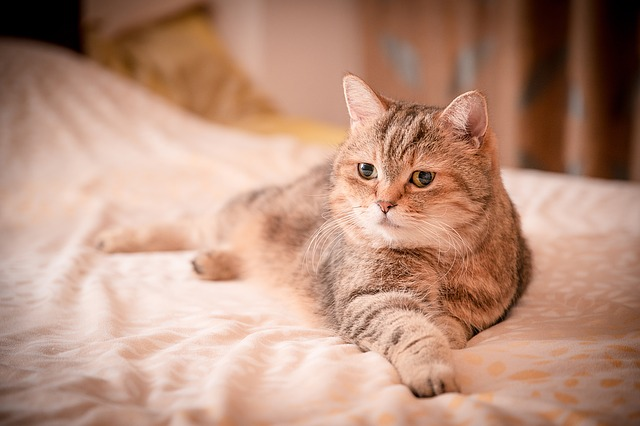
\includegraphics{images/cat}
\caption{A cat.}
\label{i:cat}
\end{figure}


樹範例如~\ref{i:tree}
\begin{figure}[!htbp]
\centering
\tikzset{every tree node/.style={align=center},
    level distance=40pt,
    sibling distance=6pt}
\begin{tikzpicture}
\Tree[.root
       [ (a) ]
       [.node
         [.node
           [ (b) ]
           [ (c) ]
         ]
         [.node
           [ (d) ]
           [ (e) ]
           [ (f) ]
           [ (g) ]
           [ (h) ]
         ]
       ]
     ]

\end{tikzpicture}

\caption{A tree. }
\label{i:tree}
\end{figure}


長條圖範例如~\ref{i:barchart}
\begin{figure}[!htbp]
    \centering
    \vspace{2em}
    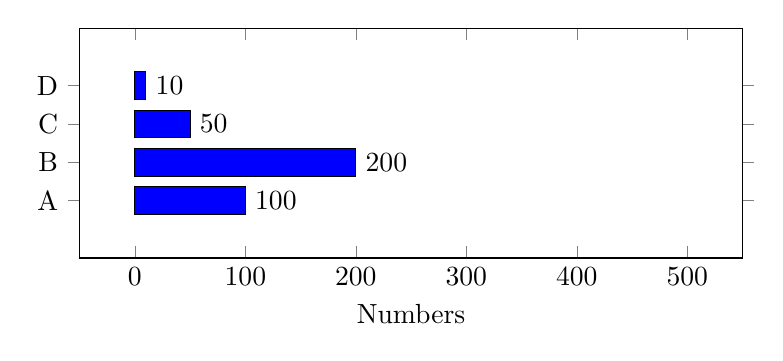
\begin{tikzpicture}
        \begin{axis}[
            enlarge y limits=0.5,
            enlarge x limits=0.1,
            height=4.5cm,
            width=10cm,
            symbolic y coords={A,B,C,D},
            xmin=0,
            xmax=500,
            xbar=1pt,
            xlabel=Numbers,
            nodes near coords={\pgfmathprintnumber[/pgf/number format/assume math mode]{\pgfplotspointmeta}},
            nodes near coords align={horizontal},
            every node near coord/.append style={
                anchor=west}
            ,
            xticklabel style={/pgf/number format/assume math mode},
            yticklabel style={/pgf/number format/assume math mode},
            ytick=data
          ]
            \addplot[xbar,fill=blue] coordinates {
            (100,A)
            (200,B)
            (50,C)
            (10,D)
            };
        \end{axis}
    \end{tikzpicture}
    \caption{A barchart.}
    \label{i:barchart}
\end{figure}



本研究分組如表~\ref{t:group}
\begin{table}[!htbp]
\centering
\caption{實驗分組}
\label{t:group}
\begin{adjustbox}{max width=\textwidth}
\begin{tabular}{@{}ccc@{}}
\toprule
\textbf{\begin{tabular}[c]{@{}c@{}}第一部分題目\\ Q1 Q2 Q3\end{tabular}} & \textbf{\begin{tabular}[c]{@{}c@{}}第二部分題目\\ Q4\end{tabular}} & \textbf{組別} \\ \midrule
abc & abc & 4 \\
abc & abc & 2 \\
abc & abc & 3 \\
abc & abc & 1 \\ \bottomrule
\end{tabular}
\end{adjustbox}
\newline
\small{資料來源:本研究}
\end{table}






    






